%!TEX root = ../dokumentation.tex
\chapter{Mechanik}

\section{Anforderungen}
Damit ein \acs{3D} Abbild eines Raumes erstellt werden kann, ist es erforderlich, dass dieser möglichst leicht in mindestens zwei Achsen beweget werden kann. Deshalb muss im Rahmen dieses Projekts eine geeignete Mechanik entworfen werden, welche es ermöglicht, den Sensor auf zwei getrennt voneinander steuerbaren Achsen beliebig positionieren zu können. Damit eine solche Mechanik entworfen werden kann müssen zuerst einige Rahmenbedingungen geklärt werden. Beispielsweiße sollten die Motoren welche die Mechanik später antreiben vorher spezifiziert sein und die maximale Größe des Sensors bekannt sein. Natürlich sollte die Mechanik auch so entworfen werden, das diese dann auch in der Praxis umgesetzt werden kann.\\
Zur besseren Visualisierung und um genaue Zeichnungen anzufertigen wurde ein \ac{CAD} Zeichenprogramm verwendet. 
\section{Entwurf}
Der gesamte Aufbau lässt sich in drei große Teile unterteilen. Einen oberen Aufbau, welcher das Kippen des Sensors übernimmt und einen Motor halten muss. Die Basis, welche sich um 360° Drehen lassen soll. Und den Rahmen, welcher die Steuerung und den zweiten Motor enthält. 

\subsection{Oberer Aufbau}
Für den oberen Aufbau der Mechanik gab es mehrere Vorraussetzungen. Zuerst soll die gesamte Mechanik so funktionieren, dass der Sensor möglichst genau im Ursprung der Dreh- und Kippachse liegt, um spätere komplizierte Umrechnungen der Punktewolke zu verhindern. Dazu soll der Aufbau möglichst leicht und klein sein, damit die Beschleunigte Masse und die damit verbundenen Trägheitskräfte möglichst gering sind, damit unnötige Belastungen auf die Motoren vermieden werden.Außerdem müssen alle Leitungen, welche in dieser Aufbaute benötigt werden 360° Drehbar sein, weshalb ein sogenannter Schleifring unumgänglich ist. 
\begin{figure}[H]
	\centering
	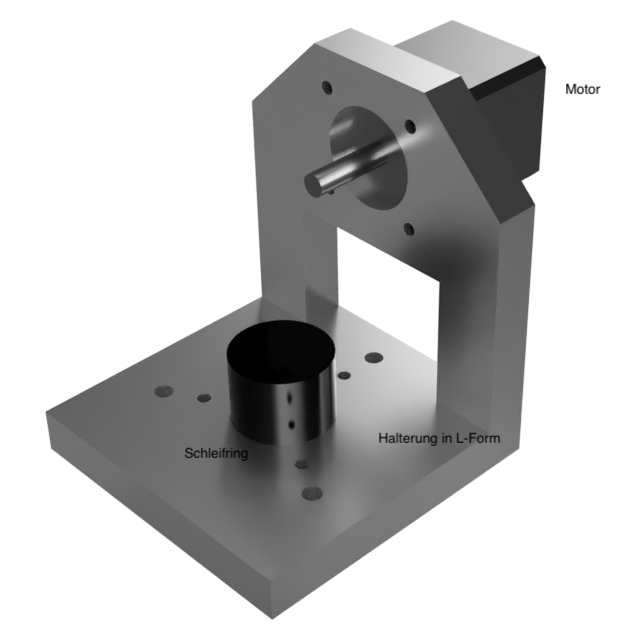
\includegraphics[width=\textwidth]{images/Mechanik/ObererAufbau}
	\caption{Oberer Aufbau der Mechanik}
	\label{obereraufbau}
\end{figure}
Der Motor welcher in Abbildung \ref{obereraufbau} zu sehen ist, ist von der \ac{NEMA} genormt und hat den Namen \ac{NEMA} 11, die 11 verweist hierbei auf die Baugröße in diesem Fall $1,1"$ was ca. $28mm$ entspricht \cite{NEMA}. Außerdem ist in der Abbildung der Schleifring zu sehen, welcher später dazu dienen wird, dass alle Kabel des Oberen Aufbaus um 360° Drehbar sind. \\
Die Halterung in L-Form besteht aus zwei Teilen, welche aneinander Geschraubt werden. Ein horizontales Teil, die Grundplatte, welche den Schleifring und die Verbindung zu den weiteren Teilen sicherstellt. Und ein vertikales Teil, welches den \ac{NEMA} 11 Motor in einer Vertiefung hält.\\
In Abbildung \ref{obereraufbau} fehlt allerdings ein weiteres Bauteil. Auf der Welle des Motors wird eine weitere Platte montiert, worauf später der \ac{LIDAR} Sensor montiert wird. Zur besseren Übersicht wurde in der gezeigten Ansicht auf diese Platte verzichtet.
\subsection{Basis}
Die Basis stellt die Verbindung zwischen dem Oberen Aufbau und dem Rahmen dar. Die Basis ist die komplexeste Baugruppe der gesamten Mechanik, da sie den Antrieb und die Lagerung des Oberen Aufbaus übernimmt. 
\begin{figure}[H]
	\centering
	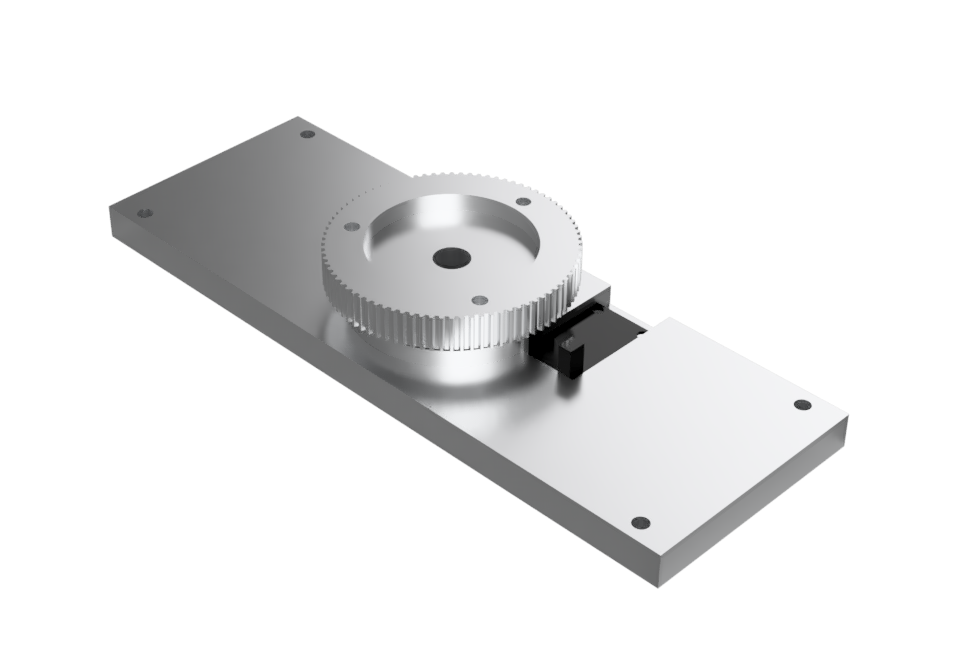
\includegraphics[width=\textwidth]{images/Mechanik/Basis}
	\caption{Basis der Mechanik}
	\label{basis}
\end{figure}
Um die Lagerung herzustellen wird ein großes Kugellager mit einem Innendurchmesser von $22mm$ in die Verbindungsplatte (Abbildung: \ref{basis}) eingepresst. Der große Innendurchmesser des Kugellagers ist erforderlich, damit die Kabel durch dieses Hindurch geführt werden können. Der Antrieb des Oberen Aufbaus wird durch eine Zahnriemenscheibe hergestellt. Diese ist nach DIN 7721-2 T2,5 \cite{Tabellenbuch} entworfen da in dieser Anwendung eine große Anzahl an Zähnen gefordert ist, um eine höhere Winkelauflösung zu erhalten, wird diese Platte 3D gedruckt werden. Um die Zahnriemenscheibe mit dem Kugellager zu verbinden wird eine Adapterplatte verwendet, welche innen in das Kugellager eingepresst wird und anschießend mit Zahnriemenscheibe und Oberem Aufbau verschraubt. Diese Adapterplatte hat ein durchgängiges Loch um die Kabel heraus zu führen. Zudem sitzt die Adapterplatte vertieft in der Zahnriemenscheibe, um die Baugröße kompakt zu halten und einen Formschluss zu erzeugen. 
\subsection{Rahmen}
Die dritte Baugruppe der Mechanik ist der Rahmen. Dieser dient hauptsächlich dazu eine stabile Befestigungsmöglichkeit für die Basis und den oberen Aufbau zu gewähren und die gesamte Elektronik zu ordnen. Zudem dient der Rahmen als Befestigungspunkt für den zweiten Motor. Der zweite Schrittmotor ist nach \ac{NEMA} 17 genormt mit einem Außenmaß von ca $41mm$. Dieser wird über einen Zahnriementrieb den gesamten oberen Aufbau um 360° Drehen. 
\begin{figure}[H]
	\centering
	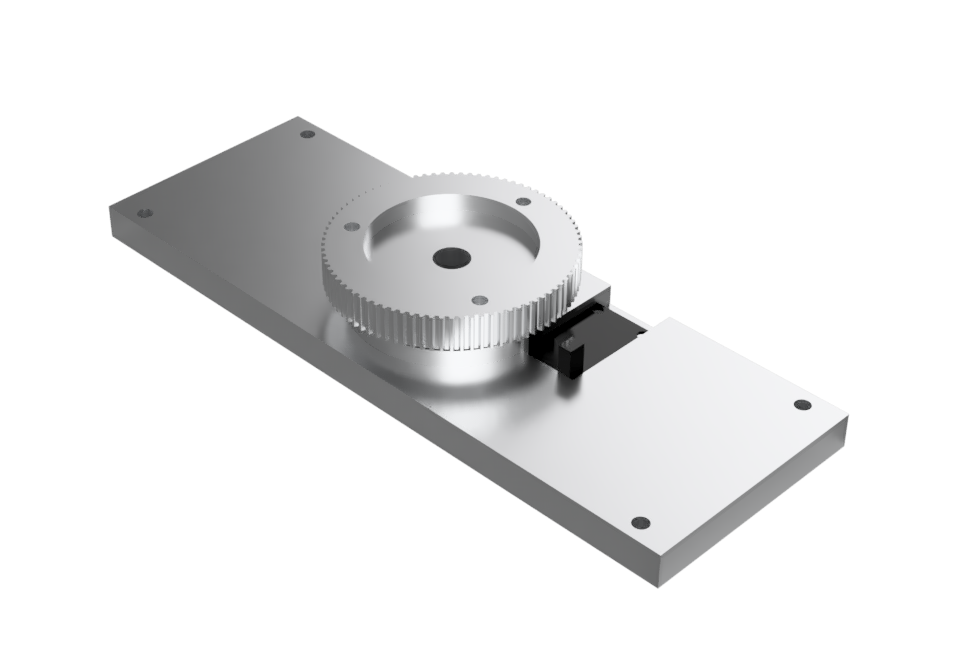
\includegraphics[width=\textwidth]{images/Mechanik/Basis}
	\caption{Motorhalterung}
	\label{motorhalterung}
\end{figure}
Um das obere Ende der Welle des zweiten Schrittmotors auf die selbe höhe wie die Oberkante der Zahnriemenscheibe zu bringen ist eine weitere Halterung erforderlich (Abbildung \ref{motorhalterung}).